% CT-1: projection is a functor — it preserves reduction, so the square commutes (a global
% step corresponds to the projected machine's step). This is why replay(trace) recovers
% state. Below: the CT-2 monoid homomorphism. Palette: global=indigo, local=teal, commute=green.
\documentclass[border=10pt]{standalone}
\usepackage{tikz}
\usepackage{amsmath}
\usepackage{amssymb}
\usepackage{xcolor}
\usetikzlibrary{arrows.meta, positioning, calc}
\definecolor{gl}{HTML}{3730A3}
\definecolor{lo}{HTML}{0D9488}
\definecolor{good}{HTML}{16A34A}
\definecolor{ink}{HTML}{1E293B}
\begin{document}
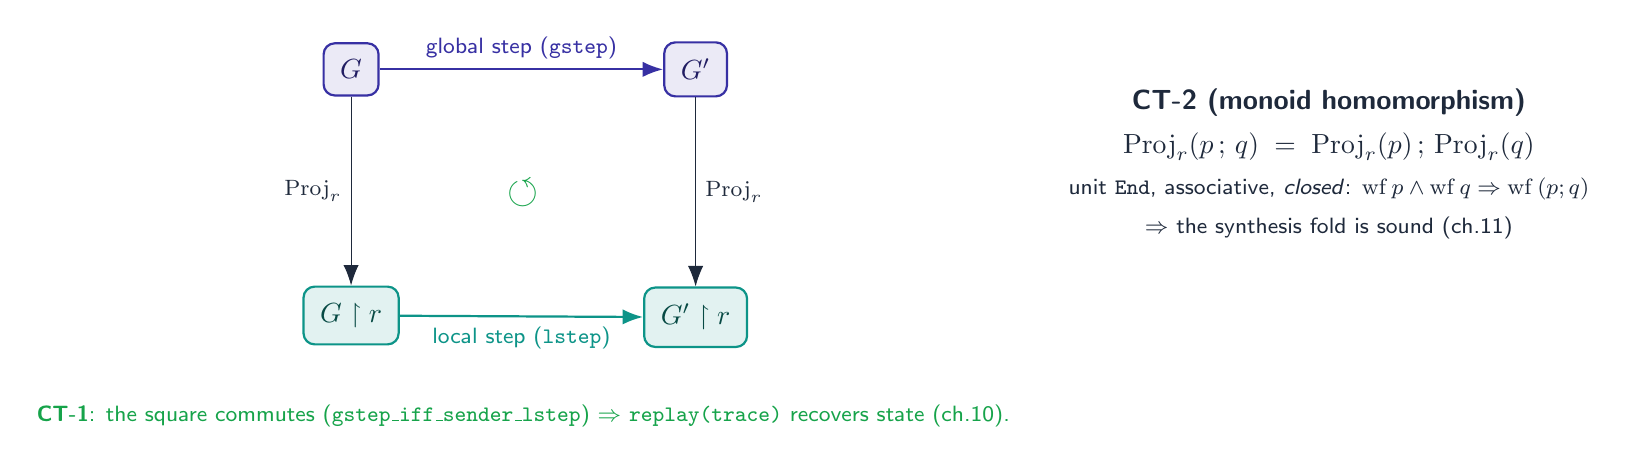
\begin{tikzpicture}[font=\sffamily, >={Latex[length=2.6mm]}, node distance=24mm and 36mm,
    g/.style={draw=gl, thick, rounded corners, fill=gl!10, inner sep=6pt, text=gl!60!black},
    l/.style={draw=lo, thick, rounded corners, fill=lo!12, inner sep=6pt, text=lo!50!black}]

  % the commuting square
  \node[g] (G)  {$G$};
  \node[g, right=of G] (G2) {$G'$};
  \node[l, below=of G]  (L)  {$G \restriction r$};
  \node[l, below=of G2] (L2) {$G' \restriction r$};

  \draw[->, gl, thick] (G) -- node[above, font=\sffamily\footnotesize]{global step (\texttt{gstep})} (G2);
  \draw[->, lo, thick] (L) -- node[below, font=\sffamily\footnotesize]{local step (\texttt{lstep})} (L2);
  \draw[->, ink] (G)  -- node[left,  font=\sffamily\footnotesize]{$\mathrm{Proj}_r$} (L);
  \draw[->, ink] (G2) -- node[right, font=\sffamily\footnotesize]{$\mathrm{Proj}_r$} (L2);
  \node[good, font=\sffamily\Large] at ($(G)!0.5!(L2)$) {$\circlearrowleft$};

  \node[good, font=\sffamily\footnotesize, align=center, below=10mm of $(L)!0.5!(L2)$]
    {\textbf{CT-1}: the square commutes (\texttt{gstep\_iff\_sender\_lstep}) $\Rightarrow$ \texttt{replay(trace)} recovers state (ch.10).};

  % CT-2 homomorphism, to the right
  \node[ink, font=\sffamily, right=42mm of G2, yshift=-12mm, align=center] (hom)
    {\textbf{CT-2 (monoid homomorphism)}\\[4pt]
     $\mathrm{Proj}_r(p \,;\, q) \;=\; \mathrm{Proj}_r(p)\,;\,\mathrm{Proj}_r(q)$\\[3pt]
     {\footnotesize unit $\mathtt{End}$, associative, \emph{closed}: $\mathrm{wf}\,p \wedge \mathrm{wf}\,q \Rightarrow \mathrm{wf}\,(p;q)$}\\[2pt]
     {\footnotesize $\Rightarrow$ the synthesis fold is sound (ch.11)}};
\end{tikzpicture}
\end{document}
